\section{Results}
\label{sec:results}

\subsection{RQ1: Feasibility and Reliability of the Genetic Algorithm}
\label{sec:rq1}

Table~\ref{tab:rq1} collects the evidence. \emph{Block-level prediction is feasible}: with the
learned weights, the first true answer is on average close to the top of the list (\textbf{MRR 0.746}),
and 84.6\% of the queries have a true answer among the first five suggestions, against an MRR of
0.118 for a random ranking. Since only 81\% of the true answers are among the candidates at all,
there is little room left at the top.

\begin{table}[ht]
\setlength{\tabcolsep}{4pt}
\begin{tabular}{@{}lcccc@{}}
\toprule
Learner & All targets & 95\% CI & Existing blocks & SD over runs \\
\midrule
\textbf{Genetic algorithm}      & \textbf{0.746} $\pm$ 0.076 & [0.727, 0.766] & \textbf{0.649} $\pm$ 0.110 & 0.0008 \\
Random search, same budget      & 0.733 $\pm$ 0.079 & [0.713, 0.754] & 0.644 $\pm$ 0.110 & 0.0031 \\
GA, negative weights allowed    & 0.742 $\pm$ 0.079 & [0.721, 0.763] & 0.641 $\pm$ 0.117 & -- \\
GA, labels shuffled in training & 0.428 $\pm$ 0.181 & [0.380, 0.476] & 0.461 $\pm$ 0.172 & -- \\
Random ranking                  & 0.118 $\pm$ 0.037 & [0.108, 0.128] & 0.116 $\pm$ 0.037 & -- \\
\bottomrule
\end{tabular}
\centering
\small
\caption{RQ1: GA evaluation (53 repositories; MRR as mean $\pm$ SD over
repositories, 95\% bootstrap CI of the mean for all targets; last column: SD of the mean over the
10 runs per fold).}
\label{tab:rq1}
\end{table}

\emph{The GA learns from the labels.} Retrained on labels shuffled within each query, it drops to
0.428, below even the unlearned equal weights (0.563), so its result comes from the relation
between signals and true answers, not from an artefact of the data. \emph{It converges reliably.}
Validation MRR rises quickly and is almost flat after 60 generations
(Figure~\ref{fig:convergence}); the mean MRR varies by only 0.0008 across the ten runs per fold, and the 27 grid
configurations by at most 0.010, so the result depends neither on the seed nor on the settings.
Allowing negative weights changes nothing (0.742) and no signal receives a negative mean weight,
which confirms the non-negativity constraint.

\emph{Against random search} with the same number of evaluations, the GA is better on 50 of 53
repositories ($p < 10^{-8}$) and four times more stable across runs, but the margin is small
(+0.013 MRR, negligible $\hat{A}_{12} = 0.56$). With only 13 continuous parameters, random sampling
already finds good weights: the GA is a useful optimizer here rather than a decisive one. The
learned weights (Figure~\ref{fig:weights}) concentrate on 3 signals: the propagation rule
(0.31), the type rule (0.20) and content similarity (0.18), with an offset of 0.21 for types to add.

\begin{figure}[ht]
\centering
\begin{subfigure}[t]{0.49\textwidth}
  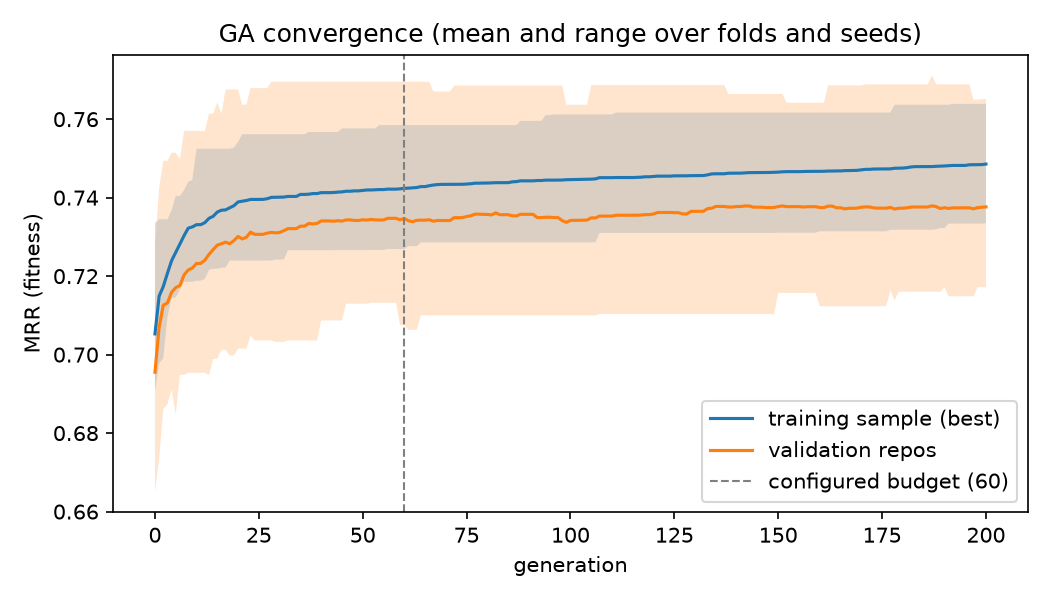
\includegraphics[width=\linewidth]{fig/convergence.png}
  \caption{Convergence: best training fitness and validation MRR per generation.}
  \label{fig:convergence}
\end{subfigure}\hfill
\begin{subfigure}[t]{0.49\textwidth}
  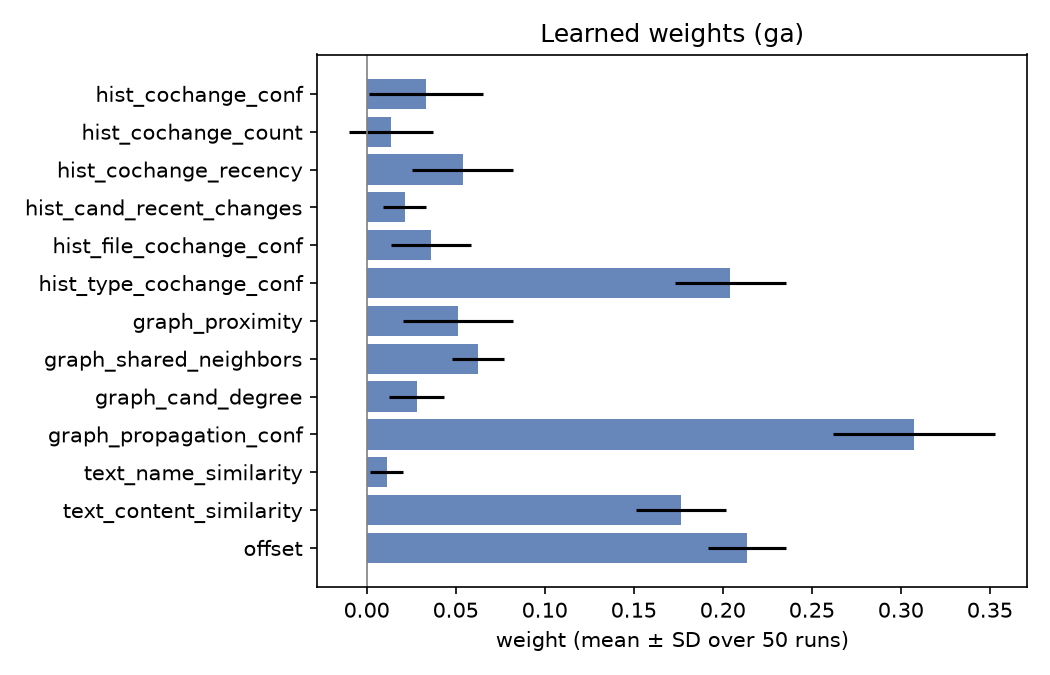
\includegraphics[width=\linewidth]{fig/learned_weights_ga.png}
  \caption{Learned weights (mean $\pm$ SD over 50 runs).}
  \label{fig:weights}
\end{subfigure}
\caption{RQ1: behavior of the Genetic Algorithm.}
\end{figure}

\subsection{RQ2: Learned Ranking vs.\ Prior Work and Equal Weights}
\label{sec:rq2}

Table~\ref{tab:rq2} compares the learned ranking with ROSE and with equal weights. On all targets
the GA is better than both on almost every repository, with large effect sizes: +0.27 MRR over ROSE
(53 of 53 repositories) and +0.18 over equal weights (51 of 53). It is also more consistent across
repositories (SD 0.076 vs.\ 0.147 for equal weights). On the 8 held-out repositories, never used
for training, it reaches 0.716, against 0.177 for equal weights.

\begin{table}[ht]
\setlength{\tabcolsep}{4pt}
\begin{tabular}{@{}llccccc@{}}
\toprule
Targets & Method & MRR & 95\% CI & MAP & Hit@5 & GA better / worse, $\hat{A}_{12}$ \\
\midrule
\multirow{3}{*}{All}
 & \textbf{GA}   & \textbf{0.746} $\pm$ 0.076 & [0.727, 0.766] & \textbf{0.437} & \textbf{0.846} & -- \\
 & Equal weights & 0.563 $\pm$ 0.147 & [0.526, 0.601] & 0.332 & 0.670 & 51 / 2, 0.87 \\
 & ROSE          & 0.481 $\pm$ 0.152 & [0.443, 0.522] & 0.231 & 0.555 & 53 / 0, 0.93 \\
\midrule
\multirow{3}{*}{Existing}
 & \textbf{GA}   & \textbf{0.649} $\pm$ 0.110 & [0.622, 0.680] & 0.439 & 0.755 & -- \\
 & Equal weights & 0.644 $\pm$ 0.106 & [0.617, 0.673] & \textbf{0.444} & \textbf{0.769} & 32 / 21, 0.52 (n.s.) \\
 & ROSE          & 0.360 $\pm$ 0.164 & [0.318, 0.405] & 0.211 & 0.440 & 53 / 0, 0.91 \\
\bottomrule
\end{tabular}
\centering
\small
\caption{RQ2: comparison with ROSE and equal weights (53 repositories; MRR as mean $\pm$ SD over
repositories with 95\% bootstrap CI). Paired tests on per-repository MRR: repositories where the GA
is better / worse and $\hat{A}_{12}$; all $p < 10^{-8}$ except where marked n.s.}
\label{tab:rq2}
\end{table}

The gain is not uniform (Figure~\ref{fig:seedaction}). It comes from \emph{added} seeds (0.732 vs.\
0.388 for equal weights), where the learned offset places the types to add correctly, and from
\emph{removed} seeds (0.853 vs.\ 0.774), driven by the propagation rule. On \emph{existing blocks}
alone the GA and equal weights are statistically tied (0.649 vs.\ 0.644, $p = 0.19$): equal
weights are already close to the best \emph{linear} combination there. ROSE stays behind everywhere
because most true answers have no earlier co-change with the seed.

\subsection{Ablation Study: Contribution of the Signal Families}
\label{sec:ablation}

To see what each signal family contributes, we retrained the GA on one family at a time (the
design of GA-IaCRec's ablation~\cite{bessghaier2026iacrec}, with learned weights; 3 runs per fold).
Every family alone is clearly worse than the combination, on all 53 repositories
(Table~\ref{tab:ablation}), and each covers a different kind of edit
(Figure~\ref{fig:ablationseed}): history carries added seeds through the type rule, the graph
carries removed seeds through the propagation rule, and text is the strongest single family for
modified seeds and on existing blocks.

\begin{table}[ht]
\setlength{\tabcolsep}{4pt}
\begin{tabular}{@{}lccccc@{}}
\toprule
Signals & All targets & 95\% CI & Existing blocks & RI (all / existing) & $\hat{A}_{12}$ (all) \\
\midrule
\textbf{GA-FULL} & \textbf{0.745} $\pm$ 0.076 & [0.727, 0.766] & \textbf{0.648} $\pm$ 0.112 & -- & -- \\
GA-HIST (6) & 0.660 $\pm$ 0.097 & [0.635, 0.685] & 0.497 $\pm$ 0.142 & +13\% / +31\% & 0.76 \\
GA-TEXT (2)    & 0.488 $\pm$ 0.162 & [0.445, 0.533] & 0.533 $\pm$ 0.145 & +53\% / +22\% & 0.92 \\
GA-GRAPH (4)   & 0.420 $\pm$ 0.112 & [0.392, 0.450] & 0.460 $\pm$ 0.114 & +78\% / +41\% & 0.99 \\
\bottomrule
\end{tabular}
\centering
\small
\caption{Ablation: the GA trained on one signal family (MRR as mean $\pm$ SD over repositories,
95\% bootstrap CI for all targets; RI = relative improvement of the full model over the variant;
full model better on 53 of 53 repositories in all targets, $p < 10^{-8}$).}
\label{tab:ablation}
\end{table}

\begin{figure}[ht]
\centering
\begin{subfigure}[t]{0.49\textwidth}
  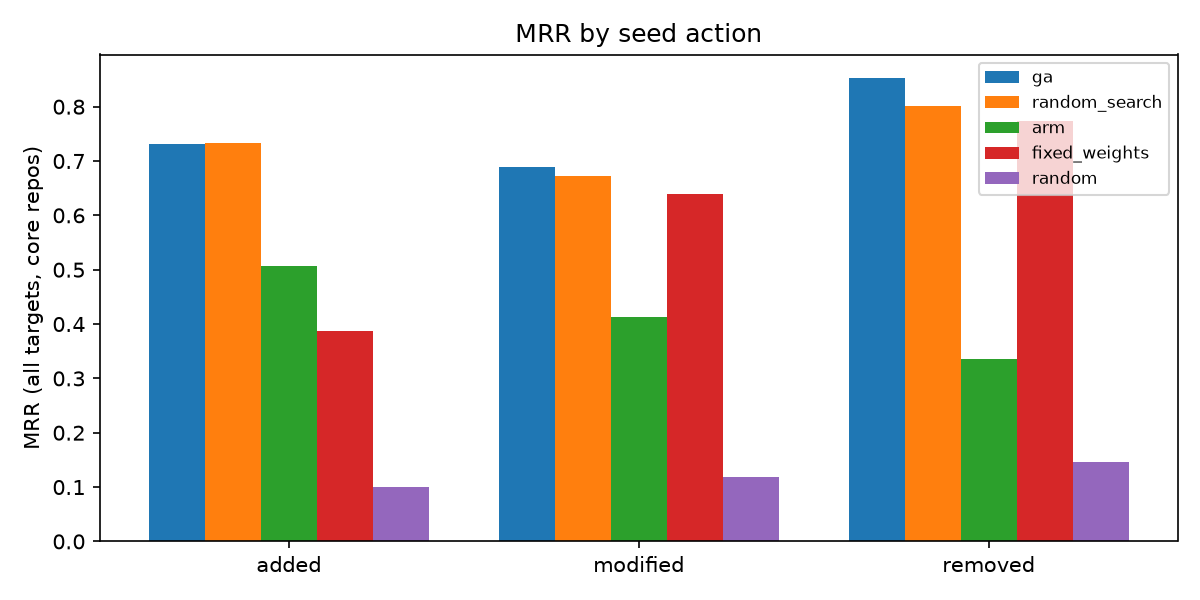
\includegraphics[width=\linewidth]{fig/mrr_by_seed_action.png}
  \caption{RQ2: GA, random search, ROSE (\texttt{arm}), equal weights (\texttt{fixed\_weights})
  and random ranking.}
  \label{fig:seedaction}
\end{subfigure}\hfill
\begin{subfigure}[t]{0.49\textwidth}
  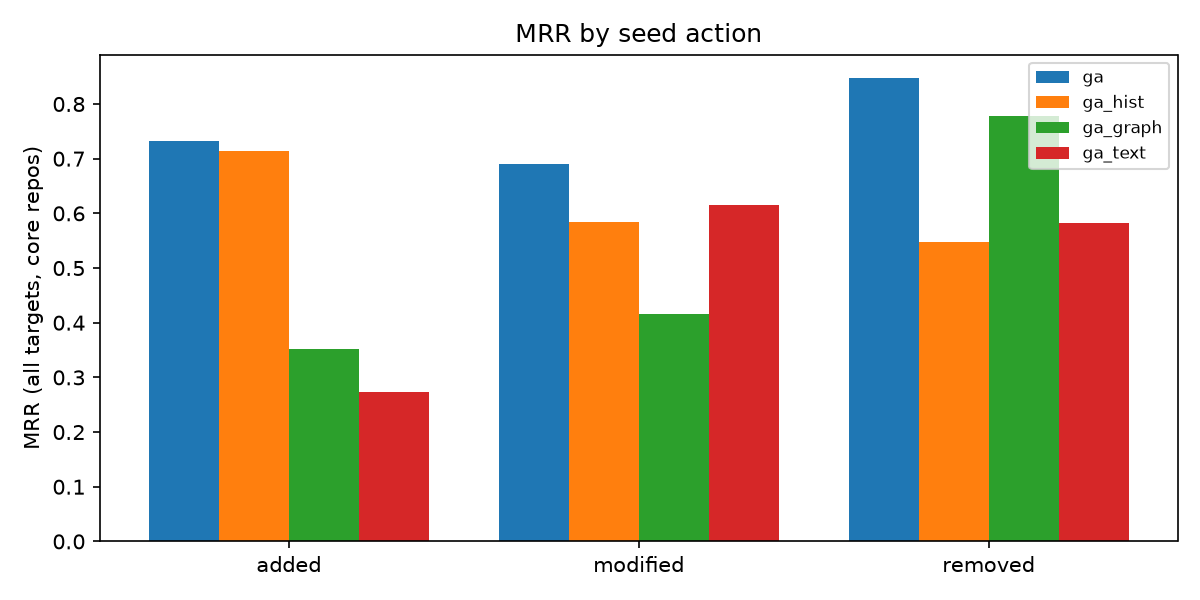
\includegraphics[width=\linewidth]{fig/ablation_seed_action.png}
  \caption{Ablation: full model vs.\ one family at a time.}
  \label{fig:ablationseed}
\end{subfigure}
\caption{MRR (all targets) by the action of the seed block.}
\end{figure}

Finally, the amount of training data matters little. Trained on 10, 25, 50 or 75\% of each fold's
training repositories, the GA reaches a test MRR of 0.734, 0.743, 0.747 and 0.744, against 0.745
with all of them: the curve is flat from about ten repositories, and training and test MRR stay
within 0.01 of each other at every size. More data would therefore not improve the model; its
linear form is the limit, which we return to in Section~\ref{sec:discussion}.
